\documentclass[10pt]{article}

\usepackage[english]{babel}
\usepackage[utf8x]{inputenc}
\usepackage{amsmath}
\usepackage{amssymb}
\usepackage{amsfonts}
\usepackage{graphicx}
\usepackage[ruled,linesnumbered,noend]{algorithm2e}
\usepackage{empheq}
\usepackage{float}
\usepackage{enumitem}
\usepackage{tikz}
\usepackage[colorlinks=true,urlcolor=blue]{hyperref}

\title{Introduction to Machine Learning, Fall 2015 - Exercise session V}
\author{Rodion ``rodde'' Efremov, student ID 013593012}

\begin{document}
 \maketitle

\section*{Problem 2 (3 points)}
\color{blue} \textit{Exclusive or} is a classical example used to demonstrate the limitations of linear classifiers. In the most basic setting, we have two binary inputs and a binary output. Using +1 and -1 as the binary values, the exclusive or function XOR is given by the following table:
\begin{center}
\begin{tabular}{|cc|c|}
$x_1$ & $x_2$ & XOR($x_1, x_2$) \\
\hline
-1 & -1 & -1 \\
-1 & +1 & +1 \\
+1 & -1 & +1 \\
+1 & +1 & -1 \\
\hline
\end{tabular}
\end{center}
\begin{itemize}
\item[(a)] Give a detailed proof for the fact that the exclusive or function cannot be represented as a linear classifier. That is, prove that there is no coefficient vector $(w_0, w_1, w_2)$ such that
\[
\text{XOR}(x_1, x_2) = \text{sign}(w_0 + w_1 x_1 + w_2 + x_2)
\]
whould hold for all possible inputs $(x_1, x_2)$.
\item[(b)] Show that if we include an extra input variable $x_1x_2$, we can represent XOR as a linear classifier in terms of the modified inputs. That is, find a coefficient vector $(w_0, w_1, w_2, w_3)$ such that
\[
\text{XOR}(x_1, x_2) = sign(w_0 + w_1 x_1 + w_2 x_2 + w_3x_1x_2)
\]
holds for all $(x_1, x_2)$.
\end{itemize}
\color{black}

\subsection*{Solution to (a)}
Define three points in $\mathbb{R}^3$:
\begin{description}
\item[$A$] $(-1, -1, w_0 - w_1 - w_2)$,
\item[$B$] $(-1, +1, w_0 - w_1 + w_2)$,
\item[$C$] $(+1, -1, w_0 + w_1 - w_2)$.
\end{description}
We must have
\begin{align*}
& w_0 - w_1 - w_2 < 0, \\
& w_0 - w_1 + w_2 > 0, \\
& w_0 + w_1 - w_2 > 0.
\end{align*}
Next, let us find a plane in $\mathbb{R}^3$ that passes through points $A, B$ and $C$: $z = ax + by + c$. Now,
\[
\begin{cases}
-a - b + c &= w_0 - w_1 - w_2 \\
-a + b + c &= w_0 - w_1 + w_2 \\
a - b + c  &= w_0 + w_1 - w_2,
\end{cases}
\]
which simplifies to
\[
\begin{cases}
-a - b + c &= w_0 - w_1 - w_2 \\
2c &= 2w_0,
\end{cases}
\]
so we have that $c = w_0$. Next,
\[
\begin{cases}
-a - b &= -w_1 - w_2 \\
-a + b & = -w_1 + w_2.
\end{cases}
\]
Which leads to $-2a = -2w_1$ and $a = w_1$, and finally $b = w_2$. Now our plane is defined as
\[
z = w_1x + w_2y + w_0.
\]
The point $D$ has coordinates $(+1, +1, w_0 + w_1 + w_2)$. Since
\begin{align*}
w_0 - w_1 + w_2 &> 0 \\
w_0 + w_1 - w_2 &> 0, \\
\end{align*}
summing the above inequalities we obtain $w_0 > 0$. Also, since $w_0 - w_1 - w_2 < 0$, we have that $w_0 < w_1 + w_2$. So $w_0 + w_1 + w_2 > 0$ and $D$ is ``misclassified'' (we should have had $w_0 + w_1 + w_2 < 0$.). 

If we chose instead of the point $D$ another point, we would get the same contradiction. The problem is that all four points do not lie on a same single plane, and this model is linear, which implies that there is no such ``desicion plane'' that could handle all four cases.

\subsection*{Solution to (b)}
This one is easy. Just define $\text{XOR}(x_1, x_2) = -\text{sign}(x_1x_2)$. Now
\begin{center}
\begin{tabular}{|c|c|c|}
\hline
$x_1$ & $x_2$ & $\text{XOR}(x_1, x_2)$ \\
\hline
-1 & -1 & $-\text{sign}((-1) \times (-1)) = -\text{sign}(1) = -1$ \\
-1 & +1 & $-\text{sign}((-1) \times (+1)) = -\text{sign}(-1) = 1$ \\
+1 & -1 & $-\text{sign}((+1) \times (-1)) = -\text{sign}(-1) = 1$ \\
+1 & +1 & $-\text{sign}((+1) \times (+1)) = -\text{sign}(1) = -1$ \\
\hline
\end{tabular}
\end{center}

\section*{Problem 3 (3 points)}
\color{blue}
\textit{Multilayer neural networks} are another way of using linear classifiers for nonlinear problems. The most basic such classifier, for two-dimensional inputs and with two \textit{hidden units}, has parameters $(u_{ij})$, $i \in \{ 1, 2 \}$, $j \in \{ 0, 1, 2 \}$ and $(v_k)$, $i \in \{ 0, 1, 2 \}$ (that is, a total of 9 parameters), and computes a mapping $(x_1, x_2) \mapsto y$ as follows:
\begin{align*}
z_1 &= \text{sign}(u_{10} + u_{11} x_1 + u_{12} x_2) \\
z_2 &= \text{sign}(u_{20} + u_{21} x_1 + u_{22} x_2) \\
7 &= \text{sign}(v_0 + v_1 z_1 + v_2 z_2). \\
\end{align*}
[The figure omitted.]
The term ``hidden unit`` refers to the computation of intermediate values $z_i$ that are not as such part of the visible input or output.
\begin{itemize}
\item[(a)] Show that with a suitable choice of the weights $(u_{ij})$ and $(v_k)$, the neural network explained aboce can compute the XOR function from Problem 2.
\item[(b)] There are numerous variants of this basic neural network model. In particular, the signum function used above in computing the values $z_i$ is often replaced by some continuous function, such as the logistic sigmoid $r \mapsto 1/(1 + e^{-r})$. However, one variant that does \textit{not} make sense is just to ignore the signum function for $z_i$ and just compute
\begin{align*}
z_1 &= u_{10} + u_{11} x_1 + u_{12} x_2 \\
z_2 &= u_{20} + u_{21} x_1 + u_{22} x_2 \\
y   &= \text{sign}(v_0 + v_1 z_1 + v_2 z_2). \\
\end{align*}
Show that this model would not offer any advantage over a basic linear classifier $y = \text{sign}(w_0 + w_1 x_1 + w_2 x_2).$
\end{itemize}
\color{black}

\subsection*{Solution to (a)}
If we restrict the values of $v_0, v_1, v_2, u_{10}, u_{11}, u_{12}, u_{20}, u_{21}, u_{22}$ to the set $\{ -1, +1 \}$, there is 16 possible assignments such that the neural network in question computes $\text{XOR}(x_1, x_2)$. One of them is
\begin{align*}
v_0 &= -1    \\
v_1 &= +1     \\
v_2 &= -1    \\
u_{10} &= +1  \\
u_{11} &= -1 \\
u_{12} &= -1 \\
u_{20} &= -1 \\
u_{21} &= -1 \\
u_{22} &= -1 \\
\end{align*}

\begin{center}
\begin{tabular}{|c|c|c|c|c|}
\hline
$x_1$ & $x_2$ & $z_1$ & $z_2$ & $y$ \\
\hline
-1 & -1 & +1 & +1 & -1 \\
-1 & +1 & +1 & -1 & +1 \\
+1 & -1 & +1 & -1 & +1 \\
+1 & +1 & -1 & -1 & -1 \\
\hline
\end{tabular}
\end{center}

\subsection*{Solution to (b)}
We have that 
\begin{align*}
y &= \text{sign}(v_0 + v_1 z_1 + v_2 z_2) \\
  &= \text{sign}(v_0 + v_1 (u_{10} + u_{11}x_1 + u_{12}x_2) + v_2 (u_{20} + u_{21}x_1 + u_{22}x_2)) \\
  &= \text{sign}(\overbrace{(v_0 + v_1 u_{10} + v_2 u_{20})}^{w_0} + \overbrace{(v_1 u_{11} + v_2 u_{21})}^{w_1} x_1 + \overbrace{(v_1 u_{12} + v_2 u_{22})}^{w_2} x_2),
\end{align*}
which is exactly what we had in Problem 2 (a).

\section*{4 (15 points)}
What comes to the (a) part, just run the Python script (013593012.py) and it will show the fitting polynomials for $K = 0, 1, \dots, 10$. The figure I got is:
\begin{figure}[H]
\begin{center}
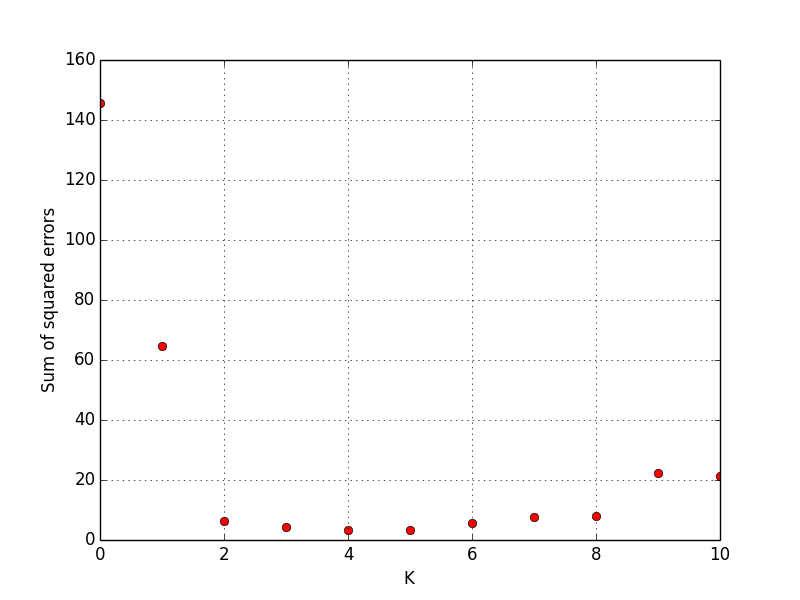
\includegraphics[scale=0.7]{CrossValidation}
\end{center}
\end{figure}
It would seem that $K = 4$ would work best, but the best $K$ varies from time to time. After $K = 5$, the error does not really improve and becomes large at $K = 9$. On another run of the program, I got that $K = 3$ is the best with sum of squared errors of $\sim 4.9$ and coefficients something like 
\[
(\overbrace{0.006}^{x^3}, \overbrace{-0.520}^{x^2}, \overbrace{0.994}^{x}, 2.019),
\] 
which is almost the target polynomial with minor ``corrections''. (\textbf{Note}: I have excluded the printing of the actual coefficients for the task (b), as there is too much of it.)
\end{document}